\documentclass{report}
\usepackage[english]{babel}
\usepackage[utf8]{inputenc}
\usepackage[T1]{fontenc}
\usepackage{listings}
\usepackage{titlesec}
\usepackage{color}
\usepackage{graphicx}
\usepackage{geometry}
\geometry{hmargin=2.5cm,vmargin=3.5cm}

\titleformat{\chapter}[display]
            {\normalfont\bfseries}{}{0pt}{\Huge}

\lstset{ escapeinside={(*}{*)} }

\title{\textbf{Rapport IHM PROG6}\\Pingouin}

\author{Castel Antonin \and Reboul Paul \and Soret Louka \and Sorin Gaëtan \and Vandendorpe Thomas \and Eymond Laritaz Cyprien}
\begin{document}

\maketitle{}
\tableofcontents
\part*{DOSSIER}

\chapter{Introduction}
bla bla bla
\chapter{Menu}
.

\section{Scenarii}
Dans le cadre de la conception de notre interface graphique, nous avons imaginé les scenarii suivants:

\begin{itemize}
\item Scenario 1
\item Scenario 2
\item Scenario 3
\item Scenario 4
\end{itemize}

(Consulter en annexes)

 
 
 %ajouter un scenario concernant la sauvegarde et le chargement des parties
 
 \subsection{ Conclusion des scenarii }
 \begin{itemize}
  \item Nous ciblons toute personne qui souhaite passer un peu de temps sur un jeu qui pourra lui offrir un défi adapté à son profil.
  \item Une connaissance sommaire des interfaces de logiciels est suffisante pour accéder au jeu dans ses règles les plus classiques. 
  \item Quelques habitudes sont un plus pour entrer plus en fond dans le jeu et avoir une expérience plus personnalisée.
  \item Savoir lire convenablement le français permet à l'utilisateur de jouer même s'il ne connaît pas les règles.
 \end{itemize}
 
 \section{ Contraintes d'ergonomie }
 
 Afin de rendre le jeu accessible aux protagonistes, nous avons conçu un menu en deux panneaux, plus un panneau de configuration pour les joueurs plus expérimentés.
 
 \paragraph{}
 Depuis chaque menu, il est possible de revenir au menu précédent ou d'accéder à un des autres menus. Un clic depuis le menu de démarrage du jeu sur le bouton "NOUVELLE PARTIE" permet d'accéder au menu de nouvelle partie où un clic sur le bouton "Config." emmène sur le panneau de configuration de la partie. D'ici, un clic sur le bouton "Retour" ramène au menu précédent, et de la même manière sur le menu de nouvelle partie, un clic sur le bouton "retour" ramène l'utilisateur sur le menu de démarrage du jeu.

%pour les espaces:
%\hspace{0.5cm}
%\vspace{0.7cm}

\chapter{Scene de jeu}
\section{Plateau}
Le plateau est évidemment l'élément principal, c'est pourquoi c'est l'élément le plus grand et qu'il est centré. Cependant beaucoup d’interactions sont possible avec ce plateau. Suite aux tests IHM,
nous avons constaté que les joueurs, lors de la première utilisation du jeu, comprennent mieux les éléments interactifs si ces derniers sont dynamiques (clignotement, mouvement, ...).

\begin{itemize}
\item Poser un pingouin: mise en évidence des cases à 1 poissons lors de la phase de pose des pingouins. La couleur de la case est de la couleur du joueur courant et clignote pour signaler un objet avec lequel on peut interragir.
  \begin{center}
    
    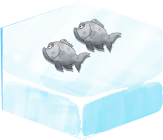
\includegraphics[width=2cm]{image/bloc_simple.png}    
    \hspace{1cm}
    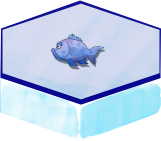
\includegraphics[width=2cm]{image/bloc_mev.png}
    \\
    bloc non cliquable \hspace{0.5cm} bloc cliquable
  \end{center}

\item Selectionner un pingouin: les pingouins sont tous identifiés par des ronds de la couleur de son joueur en dessous de lui. Nous avons ensuite rajouté une flèche sur les pingouins déplaçable du joueur courant. Ces flèches bouge indiquant qu'on peut intéragir avec le pingouin.
  \begin{center}
    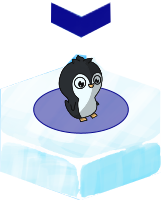
\includegraphics[width=2cm]{image/bloc_pingouin.png}    
  \end{center}
\end{itemize}

\part*{ANNEXES}

\begin{tabular}{|c|l|}
 \hline
 \multicolumn{2}{|c|}{Scenario 1}\\
 \hline
 Protagoniste(s) & Un enfant E, en âge de lire et ayant déjà utilisé une interface logicielle \\
 \hline
 Contexte(s) & \parbox{13cm} {\begin{itemize}
 	\item E est laissé seul devant un ordinateur avec le jeu des pingouins lancé en plein écran. Il ne connaît pas les règles du jeu
\end{itemize} }\\
 \hline
 Scenario & \parbox{13cm}{ E souhaite faire une partie. Il n'a aucune idée de l'existence d'une fonction pour modifier la configuration du jeu, ni ne connaît les règles. Sa connaissance de la langue française lui permet d'inférer que le bouton "NOUVELLE PARTIE" en évidence le rapproche de son objectif: démarrer une partie. \\
 Il arrive sur un panneau où il trouve trois boutons, "Config." en petit, "JOUER" en plus gros, et "Retour" en petit à nouveau. Il clique naturellement sur le bouton "JOUER", et la partie avec les règles de base se lance, à savoir 4 joueurs, dont le joueur humain qui commence, avec chacun deux pingouins. Il ne connaît pas les règles et a la présence d'esprit de regarder les éléments d'interface à sa disposition. Il tombe sur un court texte lui décrivant les actions qu'il peut faire à tout moment. En suivant les indications, il parvient à terminer sa première partie.} \\
 \hline
 \end{tabular}

\vspace{0.4cm} 
 
  \begin{tabular}{|c|l|}
  \hline
 \multicolumn{2}{|c|}{Scenario 2}\\
 \hline
 Protagoniste(s) & Une personne P plus habituée aux jeux-vidéo ou aux jeux de société \\
 \hline
 Contexte(s) & \parbox{13cm} {\begin{itemize}
 	\item P lance avec envie le jeu des pingouins dans l'optique de chercher un défi à sa hauteur
\end{itemize} }\\
 \hline
 Scenario & \parbox{13cm}{ P, de part son expérience avec les logiciels et jeux vidéos, analyse sans mal la logique de l'interface des menus après plusieurs parties, constate qu'il arrive avec une facilité déconcertante à gagner l'intégralité des parties qu'il mène. Voulant passer à la vitesse supérieure, il décide de cliquer sur les flèches près de l'image de la banquise afin de démarrer en mode "ENFER", tel que marqué dans le titre. Il joue alors contre des IA Difficiles.} \\
 \hline
 \end{tabular}
 
\vspace{0.4cm} 
 
 \begin{tabular}{|c|l|}
 \hline
 \multicolumn{2}{|c|}{Scenario 3}\\
 \hline
 Protagoniste(s) & Un habitué H qui utilise le jeu depuis un moment déjà. \\
 \hline
 Contexte(s) & \parbox{13cm} {\begin{itemize}
 	\item H utilise le jeu depuis quelques parties et pense avoir fait le tour.
 	\item H peut être P du scénario précédent, après avoir gagné ou perdu un nombre suffisamment grand pour vouloir essayer de nouvelles expériences
\end{itemize} }\\
 \hline
 Scenario & \parbox{13cm}{  Au bout d'un certain nombre de parties, H clique sur le bouton "config" afin d'explorer un monde d'options insoupçonné qui n'attendait que d'être découvert. Il découvre alors qu'il peut non seulement changer le nombre de joueurs, mais aussi leur difficulté et le nombre de leurs pingouins de manière individuelle. Il peut alors observer des matches composées uniquement d'IA si ça l'intéresse, ou même réduire le terrain de jeu à son minimum, ou encore explorer un champs de parties où le nombre de cases à trois poissons est largement supérieur au nombre des autres cases. \\
 Si H est P du scénario précédent, il sera heureux de découvrir un mode de difficulté supérieur, à savoir par exemple un nombre réduit de pingouins pour sa part par rapport à ses adversaires. Si ce dernier, en revanche a été mis en échec par les IA difficiles en mode ENFER, il pourra au contraire adapter parfaitement la difficulté à son niveau de jeu en faisant varier le nombre de pingouins et la difficulté des joueurs associés. } \\
 \hline
 \end{tabular}

\vspace{0.4cm}

\begin{tabular}{|c|l|}
\hline
 \multicolumn{2}{|c|}{Scenario 4}\\
 \hline
 Protagoniste(s) & Deux amis A1 et A2 souhaitant s'amuser entre eux avec un jeu bon enfant \\
 \hline
 Contexte(s) & \parbox{13cm} {\begin{itemize}
 	\item A1 et A2 sont à deux sur la même machine
 	\item A1 et A2 ont éventuellement une souris branchée par personne
\end{itemize} }\\
 \hline
 Scenario & \parbox{13cm}{  A1 et A2 souhaitent jouer ensemble au jeu des pingouins. Par le même procédé que le précédent, ils peuvent configurer un duel de deux joueurs humains et jouer l'un contre l'autre. \\
 Si A1 et A2 se sont renommés dans le menu de configuration en effectuant un clic droit sur "HUMAIN", ils pourront partager leurs performances avec une capture d'écran pour montrer que l'un joue mieux que son ami. \\
 Si l'un des amis joue mieux que l'autre, ils peuvent, par le même procédé que celui décrit dans le scénario précédent, permettre à l'un de poser plus de pingouins que l'autre en début de partie pour ainsi rééquilibrer leur rapport de force et ainsi rester amis.} \\
 \hline
 \end{tabular}

\end{document}
